\documentclass{article}
\usepackage[a4paper, margin=2cm]{geometry}
\usepackage{xcolor}
\usepackage{xspace}
\usepackage{booktabs}
\usepackage{dsfont}
\usepackage{footmisc}
\usepackage{marvosym}
\usepackage{amsmath}
\usepackage{hyperref}
\usepackage[capitalise,noabbrev]{cleveref}
\usepackage{tabularx}
\usepackage{listings}
\usepackage{multirow}
\usepackage{pgfplots}
\usetikzlibrary{pgfplots.statistics}
\pgfplotsset{compat=newest}

\usepgfplotslibrary{groupplots}
\pgfplotsset{every axis/.style={scale only axis}}

\definecolor{colorDirectRankStoring}{HTML}{F8BA01}
\definecolor{veryLightGrey}{HTML}{F2F2F2}
\definecolor{colorHollowTrie}{HTML}{000000}
\definecolor{colorHollowTrieDist}{HTML}{000000}
\definecolor{colorCentroidHollowTrie}{HTML}{000000}
\definecolor{colorPaCoTrieJava}{HTML}{4DAF4A}
\definecolor{colorPathDecomposedTrie}{HTML}{984EA3}
\definecolor{colorVllcp}{HTML}{E41A1C}
\definecolor{colorLcp}{HTML}{E41A1C}
\definecolor{colorTwoStepsLcp}{HTML}{E41A1C}
\definecolor{colorZFastTrieDistributor}{HTML}{377EB8}

\pgfdeclareplotmark{flippedTriangle}{%
  \pgfpathmoveto{\pgfqpointpolar{-90}{1.2\pgfplotmarksize}}%
  \pgfpathlineto{\pgfqpointpolar{30}{1.2\pgfplotmarksize}}%
  \pgfpathlineto{\pgfqpointpolar{150}{1.2\pgfplotmarksize}}%
  \pgfpathclose%
  \pgfusepath{stroke}%
}
\pgfdeclareplotmark{rightTriangle}{%
  \pgfpathmoveto{\pgfqpointpolar{0}{1.2\pgfplotmarksize}}%
  \pgfpathlineto{\pgfqpointpolar{120}{1.2\pgfplotmarksize}}%
  \pgfpathlineto{\pgfqpointpolar{240}{1.2\pgfplotmarksize}}%
  \pgfpathclose%
  \pgfusepath{stroke}%
}
\pgfdeclareplotmark{leftTriangle}{%
  \pgfpathmoveto{\pgfqpointpolar{-180}{1.2\pgfplotmarksize}}%
  \pgfpathlineto{\pgfqpointpolar{-60}{1.2\pgfplotmarksize}}%
  \pgfpathlineto{\pgfqpointpolar{60}{1.2\pgfplotmarksize}}%
  \pgfpathclose%
  \pgfusepath{stroke}%
}
\pgfdeclareimage[interpolate,height=1.85mm,width=1.85mm]{lemonMark}{fig/lemon_yellow}
\pgfdeclareplotmark{lemon}{\pgftext[at=\pgfpointorigin]{\pgfuseimage{lemonMark}}}
\pgfdeclareimage[interpolate,height=1.85mm,width=1.85mm]{lemonMarkVl}{fig/lemon_yellow_vl}
\pgfdeclareplotmark{lemonVl}{\pgftext[at=\pgfpointorigin]{\pgfuseimage{lemonMarkVl}}}

\pgfplotsset{
  major grid style={thin,dotted},
  minor grid style={thin,dotted},
  ymajorgrids,
  yminorgrids,
  every axis/.append style={
    line width=0.7pt,
    tick style={
      line cap=round,
      thin,
      major tick length=4pt,
      minor tick length=2pt,
    },
  },
  legend cell align=left,
  legend style={
    line width=0.7pt,
    /tikz/every even column/.append style={column sep=3mm,black},
    /tikz/every odd column/.append style={black},
  },
  % move title closer
  legend style={font=\small},
  title style={yshift=-2pt},
  % less space on left and right
  enlarge x limits=0.04,
  every tick label/.append style={font=\footnotesize},
  every axis label/.append style={font=\small},
  every axis y label/.append style={yshift=-1ex},
  /pgf/number format/1000 sep={},
  axis lines*=left,
  xlabel near ticks,
  ylabel near ticks,
  axis lines*=left,
  label style={font=\footnotesize},
  tick label style={font=\footnotesize},
  plotCompetitorConstruction/.style={
    title style={yshift=-15pt},
    xlabel={Bits/key},
    extra x ticks={13},
    extra x tick labels={$\geq$},
    ylabel={Constr. MKeys/s},
    xlabel shift=-5pt,
    width=70mm,
    height=50mm,
    only marks,
    xmax=13.5,
  },
  plotCompetitorQueries/.style={
    title style={yshift=-15pt},
    xlabel={Bits/key},
    ylabel={Query MKeys/s},
    extra x ticks={13},
    extra x tick labels={$\geq$},
    xlabel shift=-5pt,
    width=70mm,
    height=50mm,
    only marks,
    xmax=13.5,
  },
}

\title{GpuRecSplit plot}
\date{}
\begin{document}

% IMPORT-DATA competitors normal-distribution.txt
% IMPORT-DATA competitorNames __competitorNames.txt

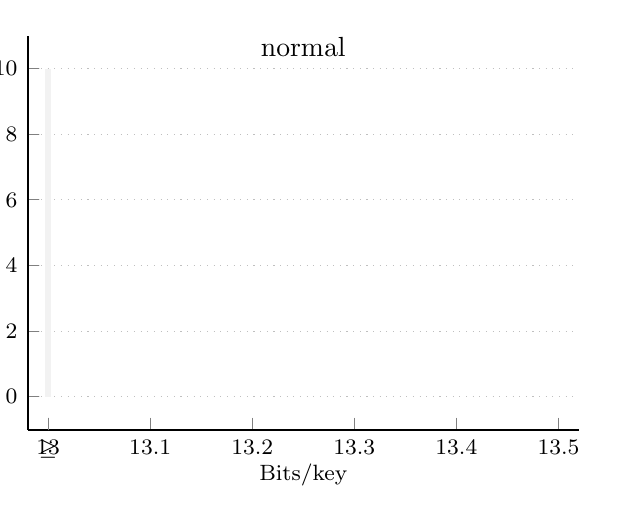
\begin{tikzpicture}[trim axis left]
    \begin{axis}[
        plotCompetitorConstruction,title={normal}
      ]
      \addplot[no marks,veryLightGrey,line width=2pt,forget plot,sharp plot] coordinates { (13,0) (13,10) };
      %% MULTIPLOT(name|ptitle|attr)
      %%   SELECT
      %%     MIN(AVG(bitsPerElement), 13) as x,
      %%     AVG(0.001*N/constructionTimeMilliseconds) as y,
      %%     name,
      %%     attr,
      %%     paper_name AS ptitle
      %%   FROM competitors
      %%   JOIN competitorNames ON name = code_name
      %%   GROUP BY name
      %%   ORDER BY name,x

      \legend{};
    \end{axis}
\end{tikzpicture}
\hfill
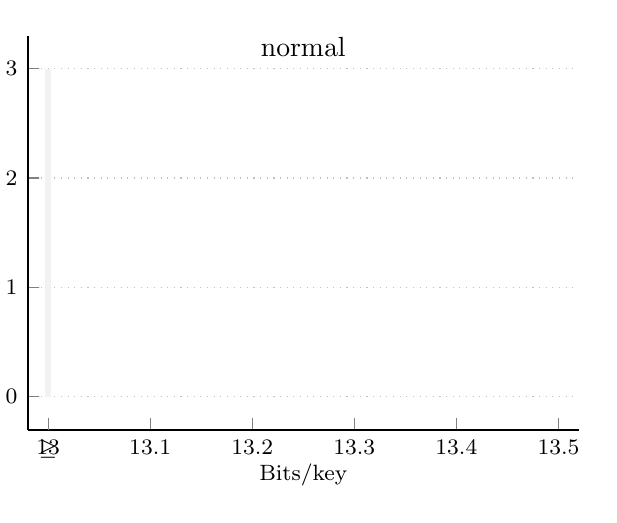
\begin{tikzpicture}[trim axis left]
    \begin{axis}[
        plotCompetitorQueries,title={normal},
        legend columns=5,
        legend to name=legend
      ]
      \addplot[no marks,veryLightGrey,line width=2pt,forget plot,sharp plot] coordinates { (13,0) (13,3) };
      %% MULTIPLOT(name|ptitle|attr)
      %%   SELECT
      %%     MIN(AVG(bitsPerElement), 13) as x,
      %%     AVG(0.001*numQueries/queryTimeMilliseconds) as y,
      %%     name,
      %%     attr,
      %%     name AS title,
      %%     paper_name AS ptitle
      %%   FROM competitors
      %%   JOIN competitorNames ON name = code_name
      %%   GROUP BY name
      %%   ORDER BY name,x

    \end{axis}
\end{tikzpicture}

\begin{tikzpicture}
    \ref*{legend}
\end{tikzpicture}

\end{document}

